% Options for packages loaded elsewhere
% Options for packages loaded elsewhere
\PassOptionsToPackage{unicode}{hyperref}
\PassOptionsToPackage{hyphens}{url}
\PassOptionsToPackage{dvipsnames,svgnames,x11names}{xcolor}
%
\documentclass[
  11pt,
  a4paper,
  onecolumn]{article}
\usepackage{xcolor}
\usepackage[top=1in,left=1in,right=1in,bottom=1in]{geometry}
\usepackage{amsmath,amssymb}
\setcounter{secnumdepth}{-\maxdimen} % remove section numbering
\usepackage{iftex}
\ifPDFTeX
  \usepackage[T1]{fontenc}
  \usepackage[utf8]{inputenc}
  \usepackage{textcomp} % provide euro and other symbols
\else % if luatex or xetex
  \usepackage{unicode-math} % this also loads fontspec
  \defaultfontfeatures{Scale=MatchLowercase}
  \defaultfontfeatures[\rmfamily]{Ligatures=TeX,Scale=1}
\fi
\usepackage{lmodern}
\ifPDFTeX\else
  % xetex/luatex font selection
\fi
% Use upquote if available, for straight quotes in verbatim environments
\IfFileExists{upquote.sty}{\usepackage{upquote}}{}
\IfFileExists{microtype.sty}{% use microtype if available
  \usepackage[]{microtype}
  \UseMicrotypeSet[protrusion]{basicmath} % disable protrusion for tt fonts
}{}
\usepackage{setspace}
\makeatletter
\@ifundefined{KOMAClassName}{% if non-KOMA class
  \IfFileExists{parskip.sty}{%
    \usepackage{parskip}
  }{% else
    \setlength{\parindent}{0pt}
    \setlength{\parskip}{6pt plus 2pt minus 1pt}}
}{% if KOMA class
  \KOMAoptions{parskip=half}}
\makeatother
% Make \paragraph and \subparagraph free-standing
\makeatletter
\ifx\paragraph\undefined\else
  \let\oldparagraph\paragraph
  \renewcommand{\paragraph}{
    \@ifstar
      \xxxParagraphStar
      \xxxParagraphNoStar
  }
  \newcommand{\xxxParagraphStar}[1]{\oldparagraph*{#1}\mbox{}}
  \newcommand{\xxxParagraphNoStar}[1]{\oldparagraph{#1}\mbox{}}
\fi
\ifx\subparagraph\undefined\else
  \let\oldsubparagraph\subparagraph
  \renewcommand{\subparagraph}{
    \@ifstar
      \xxxSubParagraphStar
      \xxxSubParagraphNoStar
  }
  \newcommand{\xxxSubParagraphStar}[1]{\oldsubparagraph*{#1}\mbox{}}
  \newcommand{\xxxSubParagraphNoStar}[1]{\oldsubparagraph{#1}\mbox{}}
\fi
\makeatother

\usepackage{color}
\usepackage{fancyvrb}
\newcommand{\VerbBar}{|}
\newcommand{\VERB}{\Verb[commandchars=\\\{\}]}
\DefineVerbatimEnvironment{Highlighting}{Verbatim}{commandchars=\\\{\}}
% Add ',fontsize=\small' for more characters per line
\newenvironment{Shaded}{}{}
\newcommand{\AlertTok}[1]{\textcolor[rgb]{1.00,0.33,0.33}{\textbf{#1}}}
\newcommand{\AnnotationTok}[1]{\textcolor[rgb]{0.42,0.45,0.49}{#1}}
\newcommand{\AttributeTok}[1]{\textcolor[rgb]{0.84,0.23,0.29}{#1}}
\newcommand{\BaseNTok}[1]{\textcolor[rgb]{0.00,0.36,0.77}{#1}}
\newcommand{\BuiltInTok}[1]{\textcolor[rgb]{0.84,0.23,0.29}{#1}}
\newcommand{\CharTok}[1]{\textcolor[rgb]{0.01,0.18,0.38}{#1}}
\newcommand{\CommentTok}[1]{\textcolor[rgb]{0.42,0.45,0.49}{#1}}
\newcommand{\CommentVarTok}[1]{\textcolor[rgb]{0.42,0.45,0.49}{#1}}
\newcommand{\ConstantTok}[1]{\textcolor[rgb]{0.00,0.36,0.77}{#1}}
\newcommand{\ControlFlowTok}[1]{\textcolor[rgb]{0.84,0.23,0.29}{#1}}
\newcommand{\DataTypeTok}[1]{\textcolor[rgb]{0.84,0.23,0.29}{#1}}
\newcommand{\DecValTok}[1]{\textcolor[rgb]{0.00,0.36,0.77}{#1}}
\newcommand{\DocumentationTok}[1]{\textcolor[rgb]{0.42,0.45,0.49}{#1}}
\newcommand{\ErrorTok}[1]{\textcolor[rgb]{1.00,0.33,0.33}{\underline{#1}}}
\newcommand{\ExtensionTok}[1]{\textcolor[rgb]{0.84,0.23,0.29}{\textbf{#1}}}
\newcommand{\FloatTok}[1]{\textcolor[rgb]{0.00,0.36,0.77}{#1}}
\newcommand{\FunctionTok}[1]{\textcolor[rgb]{0.44,0.26,0.76}{#1}}
\newcommand{\ImportTok}[1]{\textcolor[rgb]{0.01,0.18,0.38}{#1}}
\newcommand{\InformationTok}[1]{\textcolor[rgb]{0.42,0.45,0.49}{#1}}
\newcommand{\KeywordTok}[1]{\textcolor[rgb]{0.84,0.23,0.29}{#1}}
\newcommand{\NormalTok}[1]{\textcolor[rgb]{0.14,0.16,0.18}{#1}}
\newcommand{\OperatorTok}[1]{\textcolor[rgb]{0.14,0.16,0.18}{#1}}
\newcommand{\OtherTok}[1]{\textcolor[rgb]{0.44,0.26,0.76}{#1}}
\newcommand{\PreprocessorTok}[1]{\textcolor[rgb]{0.84,0.23,0.29}{#1}}
\newcommand{\RegionMarkerTok}[1]{\textcolor[rgb]{0.42,0.45,0.49}{#1}}
\newcommand{\SpecialCharTok}[1]{\textcolor[rgb]{0.00,0.36,0.77}{#1}}
\newcommand{\SpecialStringTok}[1]{\textcolor[rgb]{0.01,0.18,0.38}{#1}}
\newcommand{\StringTok}[1]{\textcolor[rgb]{0.01,0.18,0.38}{#1}}
\newcommand{\VariableTok}[1]{\textcolor[rgb]{0.89,0.38,0.04}{#1}}
\newcommand{\VerbatimStringTok}[1]{\textcolor[rgb]{0.01,0.18,0.38}{#1}}
\newcommand{\WarningTok}[1]{\textcolor[rgb]{1.00,0.33,0.33}{#1}}

\usepackage{longtable,booktabs,array}
\usepackage{calc} % for calculating minipage widths
% Correct order of tables after \paragraph or \subparagraph
\usepackage{etoolbox}
\makeatletter
\patchcmd\longtable{\par}{\if@noskipsec\mbox{}\fi\par}{}{}
\makeatother
% Allow footnotes in longtable head/foot
\IfFileExists{footnotehyper.sty}{\usepackage{footnotehyper}}{\usepackage{footnote}}
\makesavenoteenv{longtable}
\usepackage{graphicx}
\makeatletter
\newsavebox\pandoc@box
\newcommand*\pandocbounded[1]{% scales image to fit in text height/width
  \sbox\pandoc@box{#1}%
  \Gscale@div\@tempa{\textheight}{\dimexpr\ht\pandoc@box+\dp\pandoc@box\relax}%
  \Gscale@div\@tempb{\linewidth}{\wd\pandoc@box}%
  \ifdim\@tempb\p@<\@tempa\p@\let\@tempa\@tempb\fi% select the smaller of both
  \ifdim\@tempa\p@<\p@\scalebox{\@tempa}{\usebox\pandoc@box}%
  \else\usebox{\pandoc@box}%
  \fi%
}
% Set default figure placement to htbp
\def\fps@figure{htbp}
\makeatother





\setlength{\emergencystretch}{3em} % prevent overfull lines

\providecommand{\tightlist}{%
  \setlength{\itemsep}{0pt}\setlength{\parskip}{0pt}}



 


\makeatletter
\@ifpackageloaded{caption}{}{\usepackage{caption}}
\AtBeginDocument{%
\ifdefined\contentsname
  \renewcommand*\contentsname{Table of contents}
\else
  \newcommand\contentsname{Table of contents}
\fi
\ifdefined\listfigurename
  \renewcommand*\listfigurename{List of Figures}
\else
  \newcommand\listfigurename{List of Figures}
\fi
\ifdefined\listtablename
  \renewcommand*\listtablename{List of Tables}
\else
  \newcommand\listtablename{List of Tables}
\fi
\ifdefined\figurename
  \renewcommand*\figurename{Figure}
\else
  \newcommand\figurename{Figure}
\fi
\ifdefined\tablename
  \renewcommand*\tablename{Table}
\else
  \newcommand\tablename{Table}
\fi
}
\@ifpackageloaded{float}{}{\usepackage{float}}
\floatstyle{ruled}
\@ifundefined{c@chapter}{\newfloat{codelisting}{h}{lop}}{\newfloat{codelisting}{h}{lop}[chapter]}
\floatname{codelisting}{Listing}
\newcommand*\listoflistings{\listof{codelisting}{List of Listings}}
\makeatother
\makeatletter
\makeatother
\makeatletter
\@ifpackageloaded{caption}{}{\usepackage{caption}}
\@ifpackageloaded{subcaption}{}{\usepackage{subcaption}}
\makeatother
\usepackage{bookmark}
\IfFileExists{xurl.sty}{\usepackage{xurl}}{} % add URL line breaks if available
\urlstyle{same}
\hypersetup{
  pdftitle={Static PID-5 and EMA Self-Compassion},
  pdfauthor={Corrado Caudek},
  colorlinks=true,
  linkcolor={blue},
  filecolor={Maroon},
  citecolor={Blue},
  urlcolor={Blue},
  pdfcreator={LaTeX via pandoc}}


\title{Static PID-5 and EMA Self-Compassion}
\author{Corrado Caudek}
\date{}
\begin{document}
\maketitle


\setstretch{1.5}
\begin{Shaded}
\begin{Highlighting}[]
\CommentTok{\# Read and process \textquotesingle{}esi\_bf\textquotesingle{} data}
\NormalTok{esi\_bf }\OtherTok{\textless{}{-}}\NormalTok{ rio}\SpecialCharTok{::}\FunctionTok{import}\NormalTok{(}
\NormalTok{  here}\SpecialCharTok{::}\FunctionTok{here}\NormalTok{(}
    \StringTok{"data"}\NormalTok{,}
    \StringTok{"processed"}\NormalTok{,}
    \StringTok{"esi\_bf.csv"}
\NormalTok{  )}
\NormalTok{) }\SpecialCharTok{|\textgreater{}}
\NormalTok{  dplyr}\SpecialCharTok{::}\FunctionTok{distinct}\NormalTok{(user\_id, }\AttributeTok{.keep\_all =} \ConstantTok{TRUE}\NormalTok{) }\SpecialCharTok{|\textgreater{}} \CommentTok{\# Keep only distinct user\_id}
\NormalTok{  dplyr}\SpecialCharTok{::}\FunctionTok{select}\NormalTok{(user\_id, esi\_bf) }\CommentTok{\# Select relevant columns}

\CommentTok{\# Read and process \textquotesingle{}pid5\textquotesingle{} data}
\NormalTok{pid5 }\OtherTok{\textless{}{-}}\NormalTok{ rio}\SpecialCharTok{::}\FunctionTok{import}\NormalTok{(}
\NormalTok{  here}\SpecialCharTok{::}\FunctionTok{here}\NormalTok{(}
    \StringTok{"data"}\NormalTok{,}
    \StringTok{"processed"}\NormalTok{,}
    \StringTok{"pid5.csv"}
\NormalTok{  )}
\NormalTok{) }\SpecialCharTok{|\textgreater{}}
\NormalTok{  dplyr}\SpecialCharTok{::}\FunctionTok{distinct}\NormalTok{(user\_id, }\AttributeTok{.keep\_all =} \ConstantTok{TRUE}\NormalTok{) }\SpecialCharTok{|\textgreater{}}  \CommentTok{\# Keep only distinct user\_id}
\NormalTok{  dplyr}\SpecialCharTok{::}\FunctionTok{select}\NormalTok{(user\_id, }\FunctionTok{starts\_with}\NormalTok{(}\StringTok{"domain\_"}\NormalTok{)) }\CommentTok{\# Select domain variables}

\CommentTok{\# Merge \textquotesingle{}esi\_bf\textquotesingle{} and \textquotesingle{}pid5\textquotesingle{} data by user\_id}
\NormalTok{df }\OtherTok{\textless{}{-}} \FunctionTok{left\_join}\NormalTok{(esi\_bf, pid5, }\AttributeTok{by =} \StringTok{"user\_id"}\NormalTok{)}
\end{Highlighting}
\end{Shaded}

\begin{Shaded}
\begin{Highlighting}[]
\CommentTok{\# Define list of user IDs with careless responding}
\NormalTok{user\_id\_with\_careless\_responding }\OtherTok{\textless{}{-}} \FunctionTok{c}\NormalTok{(}
  \StringTok{"ma\_se\_2005\_11\_14\_490"}\NormalTok{,}
  \StringTok{"reve20041021036"}\NormalTok{,}
  \StringTok{"di\_ma\_2005\_10\_20\_756"}\NormalTok{,}
  \StringTok{"pa\_sc\_2005\_09\_10\_468"}\NormalTok{,}
  \StringTok{"il\_re\_2006\_01\_18\_645"}\NormalTok{,}
  \StringTok{"so\_ma\_2003\_10\_13\_804"}\NormalTok{,}
  \StringTok{"lo\_ca\_2005\_05\_07\_05\_437"}\NormalTok{,}
  \StringTok{"va\_ma\_2005\_05\_31\_567"}\NormalTok{,}
  \StringTok{"no\_un\_2005\_06\_29\_880"}\NormalTok{,}
  \StringTok{"an\_bo\_1988\_08\_24\_166"}\NormalTok{,}
  \StringTok{"st\_ma\_2004\_04\_21\_426"}\NormalTok{,}
  \StringTok{"an\_st\_2005\_10\_16\_052"}\NormalTok{,}
  \StringTok{"vi\_de\_2002\_12\_30\_067"}\NormalTok{,}
  \StringTok{"gi\_ru\_2005\_03\_08\_033"}\NormalTok{,}
  \StringTok{"al\_mi\_2005\_03\_05\_844"}\NormalTok{,}
  \StringTok{"la\_ma\_2006\_01\_31\_787"}\NormalTok{,}
  \StringTok{"gi\_lo\_2004\_06\_27\_237"}\NormalTok{,}
  \StringTok{"ch\_bi\_2001\_01\_28\_407"}\NormalTok{,}
  \StringTok{"al\_pe\_2001\_04\_20\_079"}\NormalTok{,}
  \StringTok{"le\_de\_2003\_09\_05\_067"}\NormalTok{,}
  \StringTok{"fe\_gr\_2002\_02\_19\_434"}\NormalTok{,}
  \StringTok{"ma\_ba\_2002\_09\_09\_052"}\NormalTok{,}
  \StringTok{"ca\_gi\_2003\_09\_16\_737"}\NormalTok{,}
  \StringTok{"an\_to\_2003\_08\_06\_114"}\NormalTok{,}
  \StringTok{"al\_se\_2003\_07\_28\_277"}\NormalTok{,}
  \StringTok{"ja\_tr\_2002\_10\_06\_487"}\NormalTok{,}
  \StringTok{"el\_ci\_2002\_02\_15\_057"}\NormalTok{,}
  \StringTok{"se\_ti\_2000\_03\_04\_975"}\NormalTok{,}
  \StringTok{"co\_ga\_2003\_10\_29\_614"}\NormalTok{,}
  \StringTok{"al\_ba\_2003\_18\_07\_905"}\NormalTok{,}
  \StringTok{"bi\_ro\_2003\_09\_07\_934"}\NormalTok{,}
  \StringTok{"an\_va\_2004\_04\_08\_527"}\NormalTok{,}
  \StringTok{"ev\_cr\_2003\_01\_27\_573"}
\NormalTok{)}

\CommentTok{\# Filter out users with careless responses}
\NormalTok{df1 }\OtherTok{\textless{}{-}}\NormalTok{ df[}\SpecialCharTok{!}\NormalTok{(df}\SpecialCharTok{$}\NormalTok{user\_id }\SpecialCharTok{\%in\%}\NormalTok{ user\_id\_with\_careless\_responding), ]}
\end{Highlighting}
\end{Shaded}

\begin{Shaded}
\begin{Highlighting}[]
\CommentTok{\# Read EMA data and rename \textquotesingle{}subj\_code\textquotesingle{} to \textquotesingle{}user\_id\textquotesingle{}}
\NormalTok{ema\_raw }\OtherTok{\textless{}{-}} \FunctionTok{readRDS}\NormalTok{(}
\NormalTok{  here}\SpecialCharTok{::}\FunctionTok{here}\NormalTok{(}
    \StringTok{"data"}\NormalTok{,}
    \StringTok{"raw"}\NormalTok{,}
    \StringTok{"ema"}\NormalTok{,}
    \StringTok{"ema\_data\_scoring.RDS"}
\NormalTok{  )}
\NormalTok{) }\SpecialCharTok{|\textgreater{}}
\NormalTok{  dplyr}\SpecialCharTok{::}\FunctionTok{rename}\NormalTok{(}
    \AttributeTok{user\_id =}\NormalTok{ subj\_code}
\NormalTok{  )}

\CommentTok{\# Merge EMA data with filtered main data}
\NormalTok{df2 }\OtherTok{\textless{}{-}} \FunctionTok{left\_join}\NormalTok{(df1, ema\_raw, }\AttributeTok{by =} \StringTok{"user\_id"}\NormalTok{)}

\CommentTok{\# Verify number of unique users}
\FunctionTok{length}\NormalTok{(}\FunctionTok{unique}\NormalTok{(df2}\SpecialCharTok{$}\NormalTok{user\_id))}
\end{Highlighting}
\end{Shaded}

\begin{verbatim}
[1] 429
\end{verbatim}

\subsection{Compliance}\label{compliance}

Escludiamo i soggetti che hanno risposto a meno di 10 notifiche.

\begin{Shaded}
\begin{Highlighting}[]
\CommentTok{\# Conta quante risposte EMA ha fornito ciascun soggetto}
\NormalTok{user\_counts }\OtherTok{\textless{}{-}}\NormalTok{ df2 }\SpecialCharTok{\%\textgreater{}\%}
  \FunctionTok{group\_by}\NormalTok{(user\_id) }\SpecialCharTok{\%\textgreater{}\%}
  \FunctionTok{summarise}\NormalTok{(}\AttributeTok{n\_responses =} \FunctionTok{n}\NormalTok{()) }\SpecialCharTok{\%\textgreater{}\%}
  \FunctionTok{ungroup}\NormalTok{()}

\CommentTok{\# Tieni solo i soggetti con almeno 10 risposte}
\NormalTok{valid\_users }\OtherTok{\textless{}{-}}\NormalTok{ user\_counts }\SpecialCharTok{\%\textgreater{}\%}
  \FunctionTok{filter}\NormalTok{(n\_responses }\SpecialCharTok{\textgreater{}=} \DecValTok{10}\NormalTok{) }\SpecialCharTok{\%\textgreater{}\%}
  \FunctionTok{pull}\NormalTok{(user\_id)}

\CommentTok{\# Filtra il dataframe originale}
\NormalTok{df2 }\OtherTok{\textless{}{-}}\NormalTok{ df2 }\SpecialCharTok{\%\textgreater{}\%}
\NormalTok{  dplyr}\SpecialCharTok{::}\FunctionTok{filter}\NormalTok{(user\_id }\SpecialCharTok{\%in\%}\NormalTok{ valid\_users)}
\end{Highlighting}
\end{Shaded}

\begin{Shaded}
\begin{Highlighting}[]
\FunctionTok{length}\NormalTok{(}\FunctionTok{unique}\NormalTok{(df2}\SpecialCharTok{$}\NormalTok{user\_id))}
\end{Highlighting}
\end{Shaded}

\begin{verbatim}
[1] 379
\end{verbatim}

\subsection{Generate negative instant
mood}\label{generate-negative-instant-mood}

\begin{Shaded}
\begin{Highlighting}[]
\CommentTok{\# Costruisce una misura media dell\textquotesingle{}affetto negativo momentaneo}

\CommentTok{\# Seleziona solo le colonne rilevanti (per velocità)}
\NormalTok{items }\OtherTok{\textless{}{-}} \FunctionTok{c}\NormalTok{(}\StringTok{"sad"}\NormalTok{, }\StringTok{"angry"}\NormalTok{, }\StringTok{"happy"}\NormalTok{, }\StringTok{"satisfied"}\NormalTok{)}

\CommentTok{\# Imputa i missing (1 solo imputazione, dato che i NA sono pochi)}
\NormalTok{imputed }\OtherTok{\textless{}{-}} \FunctionTok{mice}\NormalTok{(df2[, items], }\AttributeTok{m =} \DecValTok{1}\NormalTok{, }\AttributeTok{maxit =} \DecValTok{10}\NormalTok{, }\AttributeTok{seed =} \DecValTok{123}\NormalTok{)}
\end{Highlighting}
\end{Shaded}

\begin{verbatim}

 iter imp variable
  1   1  sad  angry  happy  satisfied
  2   1  sad  angry  happy  satisfied
  3   1  sad  angry  happy  satisfied
  4   1  sad  angry  happy  satisfied
  5   1  sad  angry  happy  satisfied
  6   1  sad  angry  happy  satisfied
  7   1  sad  angry  happy  satisfied
  8   1  sad  angry  happy  satisfied
  9   1  sad  angry  happy  satisfied
  10   1  sad  angry  happy  satisfied
\end{verbatim}

\begin{Shaded}
\begin{Highlighting}[]
\CommentTok{\# Estrai il dataset imputato e sostituisci le colonne originali}
\NormalTok{df2\_imputed }\OtherTok{\textless{}{-}} \FunctionTok{complete}\NormalTok{(imputed)}
\NormalTok{df2[, items] }\OtherTok{\textless{}{-}}\NormalTok{ df2\_imputed[, items]}

\NormalTok{df2 }\OtherTok{\textless{}{-}}\NormalTok{ df2 }\SpecialCharTok{\%\textgreater{}\%}
  \FunctionTok{mutate}\NormalTok{(}
    \AttributeTok{happy\_reversed =} \DecValTok{100} \SpecialCharTok{{-}}\NormalTok{ happy, }\CommentTok{\# Scala 0{-}100}
    \AttributeTok{satisfied\_reversed =} \DecValTok{100} \SpecialCharTok{{-}}\NormalTok{ satisfied,}
    \AttributeTok{neg\_aff\_ema =} \FunctionTok{rowMeans}\NormalTok{(}
      \FunctionTok{cbind}\NormalTok{(sad, angry, happy\_reversed, satisfied\_reversed),}
      \AttributeTok{na.rm =} \ConstantTok{TRUE}
\NormalTok{    )}
\NormalTok{  )}
\end{Highlighting}
\end{Shaded}

\subsection{Self-compassion negativa}\label{self-compassion-negativa}

Consideriamo solo le notifiche dove Self-Compassion è stata misurata.

\begin{Shaded}
\begin{Highlighting}[]
\NormalTok{df\_self\_comp\_ema }\OtherTok{\textless{}{-}}\NormalTok{ df2 }\SpecialCharTok{\%\textgreater{}\%}
\NormalTok{  dplyr}\SpecialCharTok{::}\FunctionTok{filter}\NormalTok{(}\SpecialCharTok{!}\FunctionTok{is.na}\NormalTok{(ucs\_neg) }\SpecialCharTok{\&} \SpecialCharTok{!}\FunctionTok{is.na}\NormalTok{(cs\_pos))}

\FunctionTok{length}\NormalTok{(}\FunctionTok{unique}\NormalTok{(df\_self\_comp\_ema}\SpecialCharTok{$}\NormalTok{user\_id))}
\end{Highlighting}
\end{Shaded}

\begin{verbatim}
[1] 379
\end{verbatim}

\begin{Shaded}
\begin{Highlighting}[]
\FunctionTok{dim}\NormalTok{(df\_self\_comp\_ema)}
\end{Highlighting}
\end{Shaded}

\begin{verbatim}
[1] 6229   92
\end{verbatim}

\begin{Shaded}
\begin{Highlighting}[]
\NormalTok{df\_self\_comp\_ema\_scaled }\OtherTok{\textless{}{-}}\NormalTok{ df\_self\_comp\_ema }\SpecialCharTok{\%\textgreater{}\%}
\NormalTok{  dplyr}\SpecialCharTok{::}\FunctionTok{select}\NormalTok{(}
\NormalTok{    ucs\_neg,}
\NormalTok{    domain\_negative\_affect,   }
\NormalTok{    domain\_detachment,}
\NormalTok{    domain\_antagonism,}
\NormalTok{    domain\_disinhibition,}
\NormalTok{    domain\_psychoticism,}
\NormalTok{    neg\_aff\_ema,}
\NormalTok{    pid5\_negative\_affectivity,}
\NormalTok{    pid5\_detachment,}
\NormalTok{    pid5\_antagonism,}
\NormalTok{    pid5\_disinhibition,}
\NormalTok{    pid5\_psychoticism,}
\NormalTok{    user\_id }\CommentTok{\# Mantiene user\_id così com\textquotesingle{}è}
\NormalTok{  ) }\SpecialCharTok{\%\textgreater{}\%}
\NormalTok{  dplyr}\SpecialCharTok{::}\FunctionTok{mutate}\NormalTok{(}
    \CommentTok{\# Applica la standardizzazione (scale) a tutte le colonne selezionate}
    \CommentTok{\# tranne user\_id. as.vector() è usato per assicurare che l\textquotesingle{}output sia un vettore.}
\NormalTok{    dplyr}\SpecialCharTok{::}\FunctionTok{across}\NormalTok{(}
      \FunctionTok{c}\NormalTok{(}
\NormalTok{        ucs\_neg,}
\NormalTok{        neg\_aff\_ema,}
\NormalTok{        domain\_negative\_affect,   }
\NormalTok{        domain\_detachment,}
\NormalTok{        domain\_antagonism,}
\NormalTok{        domain\_disinhibition,}
\NormalTok{        domain\_psychoticism,}
\NormalTok{        pid5\_negative\_affectivity,}
\NormalTok{        pid5\_detachment,}
\NormalTok{        pid5\_antagonism,}
\NormalTok{        pid5\_disinhibition,}
\NormalTok{        pid5\_psychoticism}
\NormalTok{      ),}
      \SpecialCharTok{\textasciitilde{}} \FunctionTok{as.vector}\NormalTok{(}\FunctionTok{scale}\NormalTok{(.))}
\NormalTok{    )}
\NormalTok{  )}
\end{Highlighting}
\end{Shaded}

\begin{Shaded}
\begin{Highlighting}[]
\NormalTok{model\_base }\OtherTok{\textless{}{-}} \FunctionTok{brm}\NormalTok{(}
\NormalTok{  ucs\_neg }\SpecialCharTok{\textasciitilde{}}\NormalTok{ neg\_aff\_ema }\SpecialCharTok{+} 
\NormalTok{    domain\_negative\_affect }\SpecialCharTok{+}\NormalTok{ domain\_detachment }\SpecialCharTok{+}
\NormalTok{    domain\_antagonism }\SpecialCharTok{+}\NormalTok{ domain\_disinhibition }\SpecialCharTok{+}\NormalTok{ domain\_psychoticism }\SpecialCharTok{+} 
\NormalTok{    (}\DecValTok{1} \SpecialCharTok{+}\NormalTok{ neg\_aff\_ema }\SpecialCharTok{|}\NormalTok{ user\_id),}
  \AttributeTok{data =}\NormalTok{ df\_self\_comp\_ema\_scaled,}
  \AttributeTok{family =} \FunctionTok{skew\_normal}\NormalTok{(),}
  \AttributeTok{prior =} \FunctionTok{c}\NormalTok{(}
    \FunctionTok{prior}\NormalTok{(}\FunctionTok{normal}\NormalTok{(}\DecValTok{0}\NormalTok{, }\DecValTok{1}\NormalTok{), }\AttributeTok{class =} \StringTok{"Intercept"}\NormalTok{),}
    \FunctionTok{prior}\NormalTok{(}\FunctionTok{normal}\NormalTok{(}\DecValTok{0}\NormalTok{, }\DecValTok{1}\NormalTok{), }\AttributeTok{class =} \StringTok{"b"}\NormalTok{),}
    \FunctionTok{prior}\NormalTok{(}\FunctionTok{exponential}\NormalTok{(}\DecValTok{1}\NormalTok{), }\AttributeTok{class =} \StringTok{"sd"}\NormalTok{),}
    \FunctionTok{prior}\NormalTok{(}\FunctionTok{exponential}\NormalTok{(}\DecValTok{1}\NormalTok{), }\AttributeTok{class =} \StringTok{"sigma"}\NormalTok{)}
\NormalTok{  ),}
  \AttributeTok{chains =} \DecValTok{4}\NormalTok{,}
  \AttributeTok{cores =} \DecValTok{4}\NormalTok{,}
  \AttributeTok{iter =} \DecValTok{2000}\NormalTok{,}
  \AttributeTok{seed =} \DecValTok{123}\NormalTok{,}
  \AttributeTok{backend =} \StringTok{"cmdstanr"}\NormalTok{,}
  \AttributeTok{save\_pars =} \FunctionTok{save\_pars}\NormalTok{(}\AttributeTok{all =} \ConstantTok{TRUE}\NormalTok{)}
\NormalTok{)}
\end{Highlighting}
\end{Shaded}

\begin{Shaded}
\begin{Highlighting}[]
\CommentTok{\# Posterior predictive check for the baseline model}
\FunctionTok{pp\_check}\NormalTok{(model\_base)}
\end{Highlighting}
\end{Shaded}

\begin{verbatim}
Using 10 posterior draws for ppc type 'dens_overlay' by default.
\end{verbatim}

\pandocbounded{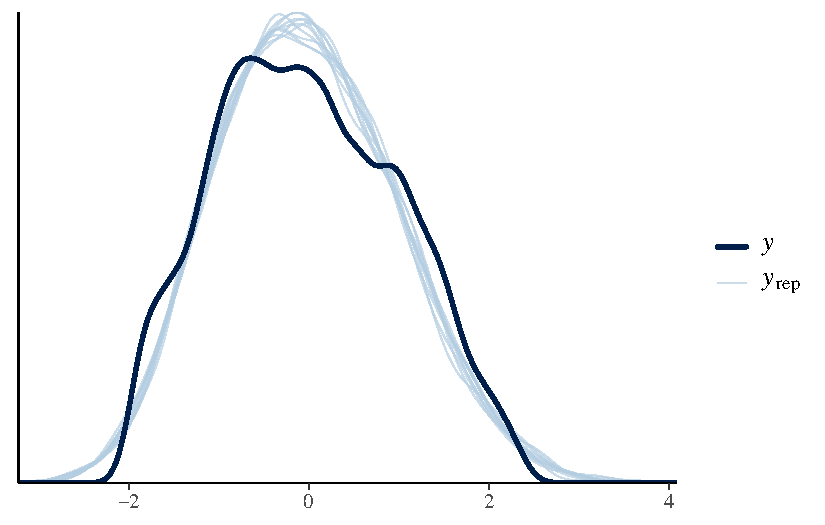
\includegraphics[keepaspectratio]{pid5_self_compassion_1_files/figure-pdf/unnamed-chunk-12-1.pdf}}

\begin{Shaded}
\begin{Highlighting}[]
\FunctionTok{print}\NormalTok{(model\_base)}
\end{Highlighting}
\end{Shaded}

\begin{verbatim}
 Family: skew_normal 
  Links: mu = identity; sigma = identity; alpha = identity 
Formula: ucs_neg ~ neg_aff_ema + domain_negative_affect + domain_detachment + domain_antagonism + domain_disinhibition + domain_psychoticism + (1 + neg_aff_ema | user_id) 
   Data: df_self_comp_ema_scaled (Number of observations: 5757) 
  Draws: 4 chains, each with iter = 2000; warmup = 1000; thin = 1;
         total post-warmup draws = 4000

Multilevel Hyperparameters:
~user_id (Number of levels: 350) 
                           Estimate Est.Error l-95% CI u-95% CI Rhat Bulk_ESS
sd(Intercept)                  0.52      0.02     0.48     0.57 1.00      731
sd(neg_aff_ema)                0.21      0.01     0.18     0.24 1.00     1449
cor(Intercept,neg_aff_ema)     0.16      0.08     0.00     0.31 1.00     1272
                           Tail_ESS
sd(Intercept)                  1395
sd(neg_aff_ema)                2295
cor(Intercept,neg_aff_ema)     2424

Regression Coefficients:
                       Estimate Est.Error l-95% CI u-95% CI Rhat Bulk_ESS
Intercept                 -0.02      0.03    -0.08     0.04 1.01      357
neg_aff_ema                0.36      0.02     0.33     0.40 1.00     2015
domain_negative_affect     0.31      0.04     0.24     0.38 1.01      467
domain_detachment          0.05      0.03    -0.01     0.12 1.01      599
domain_antagonism          0.00      0.03    -0.06     0.07 1.01      486
domain_disinhibition       0.09      0.04     0.01     0.16 1.01      558
domain_psychoticism        0.02      0.04    -0.06     0.10 1.01      546
                       Tail_ESS
Intercept                   656
neg_aff_ema                2567
domain_negative_affect     1076
domain_detachment           926
domain_antagonism           923
domain_disinhibition       1168
domain_psychoticism         981

Further Distributional Parameters:
      Estimate Est.Error l-95% CI u-95% CI Rhat Bulk_ESS Tail_ESS
sigma     0.58      0.01     0.56     0.59 1.00     4331     2848
alpha     1.28      0.11     1.05     1.49 1.00     3844     3176

Draws were sampled using sample(hmc). For each parameter, Bulk_ESS
and Tail_ESS are effective sample size measures, and Rhat is the potential
scale reduction factor on split chains (at convergence, Rhat = 1).
\end{verbatim}

\begin{Shaded}
\begin{Highlighting}[]
\CommentTok{\# Fit augmented Bayesian model with interaction effects}
\NormalTok{model\_alt }\OtherTok{\textless{}{-}} \FunctionTok{brm}\NormalTok{(}
\NormalTok{  ucs\_neg }\SpecialCharTok{\textasciitilde{}}
\NormalTok{    (neg\_aff\_ema }\SpecialCharTok{+}\NormalTok{ domain\_negative\_affect }\SpecialCharTok{+}\NormalTok{ domain\_detachment }\SpecialCharTok{+} 
\NormalTok{       domain\_antagonism }\SpecialCharTok{+}\NormalTok{ domain\_disinhibition }\SpecialCharTok{+}\NormalTok{ domain\_psychoticism) }\SpecialCharTok{*}
\NormalTok{      (pid5\_negative\_affectivity }\SpecialCharTok{+}\NormalTok{ pid5\_detachment }\SpecialCharTok{+}\NormalTok{ pid5\_antagonism }\SpecialCharTok{+}
\NormalTok{         pid5\_disinhibition }\SpecialCharTok{+}\NormalTok{ pid5\_psychoticism) }\SpecialCharTok{+}
\NormalTok{    (}\DecValTok{1} \SpecialCharTok{+}\NormalTok{ neg\_aff\_ema }\SpecialCharTok{|}\NormalTok{ user\_id),}
  \AttributeTok{data =}\NormalTok{ df\_self\_comp\_ema\_scaled,}
  \AttributeTok{family =} \FunctionTok{skew\_normal}\NormalTok{(),}
  \AttributeTok{prior =} \FunctionTok{c}\NormalTok{(}
    \FunctionTok{prior}\NormalTok{(}\FunctionTok{normal}\NormalTok{(}\DecValTok{0}\NormalTok{, }\DecValTok{1}\NormalTok{), }\AttributeTok{class =} \StringTok{"Intercept"}\NormalTok{),}
    \FunctionTok{prior}\NormalTok{(}\FunctionTok{normal}\NormalTok{(}\DecValTok{0}\NormalTok{, }\DecValTok{1}\NormalTok{), }\AttributeTok{class =} \StringTok{"b"}\NormalTok{),}
    \FunctionTok{prior}\NormalTok{(}\FunctionTok{exponential}\NormalTok{(}\DecValTok{1}\NormalTok{), }\AttributeTok{class =} \StringTok{"sd"}\NormalTok{),}
    \FunctionTok{prior}\NormalTok{(}\FunctionTok{exponential}\NormalTok{(}\DecValTok{1}\NormalTok{), }\AttributeTok{class =} \StringTok{"sigma"}\NormalTok{)}
\NormalTok{  ),}
  \AttributeTok{chains =} \DecValTok{4}\NormalTok{,}
  \AttributeTok{cores =} \DecValTok{4}\NormalTok{,}
  \AttributeTok{iter =} \DecValTok{2000}\NormalTok{,}
  \AttributeTok{seed =} \DecValTok{123}\NormalTok{,}
  \AttributeTok{backend =} \StringTok{"cmdstanr"}\NormalTok{,}
  \AttributeTok{save\_pars =} \FunctionTok{save\_pars}\NormalTok{(}\AttributeTok{all =} \ConstantTok{TRUE}\NormalTok{)}
\NormalTok{)}
\end{Highlighting}
\end{Shaded}

\begin{Shaded}
\begin{Highlighting}[]
\FunctionTok{pp\_check}\NormalTok{(model\_alt)}
\end{Highlighting}
\end{Shaded}

\begin{verbatim}
Using 10 posterior draws for ppc type 'dens_overlay' by default.
\end{verbatim}

\pandocbounded{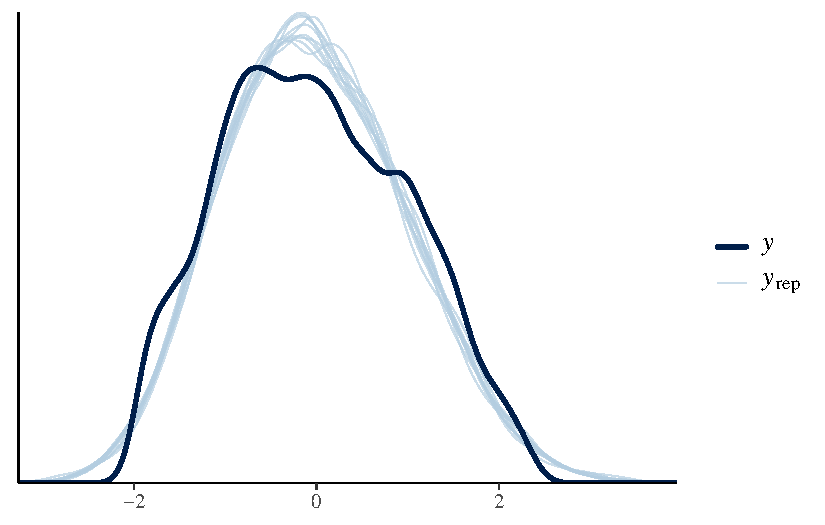
\includegraphics[keepaspectratio]{pid5_self_compassion_1_files/figure-pdf/unnamed-chunk-15-1.pdf}}

\begin{Shaded}
\begin{Highlighting}[]
\FunctionTok{print}\NormalTok{(model\_alt)}
\end{Highlighting}
\end{Shaded}

\begin{verbatim}
 Family: skew_normal 
  Links: mu = identity; sigma = identity; alpha = identity 
Formula: ucs_neg ~ (neg_aff_ema + domain_negative_affect + domain_detachment + domain_antagonism + domain_disinhibition + domain_psychoticism) * (pid5_negative_affectivity + pid5_detachment + pid5_antagonism + pid5_disinhibition + pid5_psychoticism) + (1 + neg_aff_ema | user_id) 
   Data: df_self_comp_ema_scaled (Number of observations: 5757) 
  Draws: 4 chains, each with iter = 2000; warmup = 1000; thin = 1;
         total post-warmup draws = 4000

Multilevel Hyperparameters:
~user_id (Number of levels: 350) 
                           Estimate Est.Error l-95% CI u-95% CI Rhat Bulk_ESS
sd(Intercept)                  0.39      0.02     0.36     0.42 1.01     1006
sd(neg_aff_ema)                0.13      0.01     0.11     0.16 1.00     1047
cor(Intercept,neg_aff_ema)     0.24      0.10     0.04     0.43 1.00     1554
                           Tail_ESS
sd(Intercept)                  1868
sd(neg_aff_ema)                2069
cor(Intercept,neg_aff_ema)     1943

Regression Coefficients:
                                                 Estimate Est.Error l-95% CI
Intercept                                           -0.03      0.02    -0.08
neg_aff_ema                                          0.19      0.01     0.16
domain_negative_affect                               0.20      0.03     0.15
domain_detachment                                    0.03      0.03    -0.03
domain_antagonism                                    0.00      0.03    -0.05
domain_disinhibition                                 0.05      0.03    -0.01
domain_psychoticism                                 -0.01      0.03    -0.08
pid5_negative_affectivity                            0.28      0.01     0.26
pid5_detachment                                      0.13      0.01     0.10
pid5_antagonism                                     -0.09      0.01    -0.12
pid5_disinhibition                                   0.15      0.01     0.13
pid5_psychoticism                                    0.04      0.02     0.01
neg_aff_ema:pid5_negative_affectivity               -0.00      0.01    -0.02
neg_aff_ema:pid5_detachment                         -0.02      0.01    -0.04
neg_aff_ema:pid5_antagonism                         -0.01      0.01    -0.03
neg_aff_ema:pid5_disinhibition                       0.03      0.01     0.02
neg_aff_ema:pid5_psychoticism                       -0.02      0.01    -0.04
domain_negative_affect:pid5_negative_affectivity     0.06      0.01     0.03
domain_negative_affect:pid5_detachment               0.02      0.01    -0.01
domain_negative_affect:pid5_antagonism              -0.02      0.01    -0.05
domain_negative_affect:pid5_disinhibition           -0.04      0.01    -0.06
domain_negative_affect:pid5_psychoticism            -0.02      0.02    -0.05
domain_detachment:pid5_negative_affectivity          0.01      0.01    -0.02
domain_detachment:pid5_detachment                   -0.00      0.01    -0.03
domain_detachment:pid5_antagonism                    0.01      0.01    -0.02
domain_detachment:pid5_disinhibition                -0.01      0.01    -0.03
domain_detachment:pid5_psychoticism                 -0.00      0.01    -0.03
domain_antagonism:pid5_negative_affectivity         -0.00      0.01    -0.03
domain_antagonism:pid5_detachment                   -0.02      0.01    -0.05
domain_antagonism:pid5_antagonism                    0.03      0.01     0.01
domain_antagonism:pid5_disinhibition                -0.02      0.01    -0.04
domain_antagonism:pid5_psychoticism                 -0.01      0.01    -0.03
domain_disinhibition:pid5_negative_affectivity      -0.01      0.01    -0.03
domain_disinhibition:pid5_detachment                 0.00      0.01    -0.03
domain_disinhibition:pid5_antagonism                -0.02      0.01    -0.05
domain_disinhibition:pid5_disinhibition              0.02      0.01    -0.01
domain_disinhibition:pid5_psychoticism              -0.01      0.01    -0.04
domain_psychoticism:pid5_negative_affectivity        0.01      0.02    -0.02
domain_psychoticism:pid5_detachment                 -0.01      0.02    -0.04
domain_psychoticism:pid5_antagonism                 -0.01      0.01    -0.03
domain_psychoticism:pid5_disinhibition               0.01      0.01    -0.02
domain_psychoticism:pid5_psychoticism                0.01      0.02    -0.02
                                                 u-95% CI Rhat Bulk_ESS
Intercept                                            0.01 1.01      689
neg_aff_ema                                          0.21 1.00     2272
domain_negative_affect                               0.26 1.00      755
domain_detachment                                    0.08 1.01      481
domain_antagonism                                    0.05 1.00      661
domain_disinhibition                                 0.11 1.00      723
domain_psychoticism                                  0.05 1.01      485
pid5_negative_affectivity                            0.31 1.00     3004
pid5_detachment                                      0.16 1.00     3156
pid5_antagonism                                     -0.07 1.00     2915
pid5_disinhibition                                   0.17 1.00     3902
pid5_psychoticism                                    0.07 1.00     2931
neg_aff_ema:pid5_negative_affectivity                0.02 1.00     3792
neg_aff_ema:pid5_detachment                         -0.00 1.00     3517
neg_aff_ema:pid5_antagonism                          0.01 1.00     4201
neg_aff_ema:pid5_disinhibition                       0.05 1.00     3971
neg_aff_ema:pid5_psychoticism                        0.01 1.00     3551
domain_negative_affect:pid5_negative_affectivity     0.08 1.00     2855
domain_negative_affect:pid5_detachment               0.05 1.00     2256
domain_negative_affect:pid5_antagonism               0.01 1.00     2770
domain_negative_affect:pid5_disinhibition           -0.01 1.00     3479
domain_negative_affect:pid5_psychoticism             0.02 1.00     2156
domain_detachment:pid5_negative_affectivity          0.04 1.00     3000
domain_detachment:pid5_detachment                    0.03 1.00     2743
domain_detachment:pid5_antagonism                    0.03 1.00     2991
domain_detachment:pid5_disinhibition                 0.02 1.00     3364
domain_detachment:pid5_psychoticism                  0.02 1.00     2538
domain_antagonism:pid5_negative_affectivity          0.02 1.00     2562
domain_antagonism:pid5_detachment                    0.00 1.00     2769
domain_antagonism:pid5_antagonism                    0.06 1.00     2740
domain_antagonism:pid5_disinhibition                 0.01 1.00     3406
domain_antagonism:pid5_psychoticism                  0.02 1.00     2748
domain_disinhibition:pid5_negative_affectivity       0.02 1.00     2799
domain_disinhibition:pid5_detachment                 0.03 1.00     2435
domain_disinhibition:pid5_antagonism                -0.00 1.00     3241
domain_disinhibition:pid5_disinhibition              0.04 1.00     3537
domain_disinhibition:pid5_psychoticism               0.02 1.00     2704
domain_psychoticism:pid5_negative_affectivity        0.04 1.00     2228
domain_psychoticism:pid5_detachment                  0.02 1.00     2184
domain_psychoticism:pid5_antagonism                  0.02 1.00     2766
domain_psychoticism:pid5_disinhibition               0.04 1.00     3107
domain_psychoticism:pid5_psychoticism                0.04 1.00     2278
                                                 Tail_ESS
Intercept                                            1542
neg_aff_ema                                          3434
domain_negative_affect                               1384
domain_detachment                                    1055
domain_antagonism                                    1420
domain_disinhibition                                 1438
domain_psychoticism                                  1048
pid5_negative_affectivity                            2991
pid5_detachment                                      3020
pid5_antagonism                                      3262
pid5_disinhibition                                   3392
pid5_psychoticism                                    2676
neg_aff_ema:pid5_negative_affectivity                3398
neg_aff_ema:pid5_detachment                          2727
neg_aff_ema:pid5_antagonism                          3087
neg_aff_ema:pid5_disinhibition                       3185
neg_aff_ema:pid5_psychoticism                        3221
domain_negative_affect:pid5_negative_affectivity     3292
domain_negative_affect:pid5_detachment               3138
domain_negative_affect:pid5_antagonism               2935
domain_negative_affect:pid5_disinhibition            2941
domain_negative_affect:pid5_psychoticism             2969
domain_detachment:pid5_negative_affectivity          2873
domain_detachment:pid5_detachment                    3118
domain_detachment:pid5_antagonism                    3143
domain_detachment:pid5_disinhibition                 2914
domain_detachment:pid5_psychoticism                  2816
domain_antagonism:pid5_negative_affectivity          2666
domain_antagonism:pid5_detachment                    3164
domain_antagonism:pid5_antagonism                    3109
domain_antagonism:pid5_disinhibition                 3514
domain_antagonism:pid5_psychoticism                  2884
domain_disinhibition:pid5_negative_affectivity       2992
domain_disinhibition:pid5_detachment                 2897
domain_disinhibition:pid5_antagonism                 3189
domain_disinhibition:pid5_disinhibition              2794
domain_disinhibition:pid5_psychoticism               2991
domain_psychoticism:pid5_negative_affectivity        2745
domain_psychoticism:pid5_detachment                  2840
domain_psychoticism:pid5_antagonism                  3363
domain_psychoticism:pid5_disinhibition               2770
domain_psychoticism:pid5_psychoticism                2468

Further Distributional Parameters:
      Estimate Est.Error l-95% CI u-95% CI Rhat Bulk_ESS Tail_ESS
sigma     0.53      0.01     0.52     0.54 1.00     4476     2921
alpha     1.20      0.11     0.97     1.42 1.00     2977     2787

Draws were sampled using sample(hmc). For each parameter, Bulk_ESS
and Tail_ESS are effective sample size measures, and Rhat is the potential
scale reduction factor on split chains (at convergence, Rhat = 1).
\end{verbatim}

\begin{Shaded}
\begin{Highlighting}[]
\NormalTok{loo0 }\OtherTok{\textless{}{-}} \FunctionTok{loo}\NormalTok{(model\_base, }\AttributeTok{save\_psis =} \ConstantTok{TRUE}\NormalTok{)}
\end{Highlighting}
\end{Shaded}

\begin{verbatim}
Warning: Found 10 observations with a pareto_k > 0.7 in model 'model_base'. We
recommend to set 'moment_match = TRUE' in order to perform moment matching for
problematic observations.
\end{verbatim}

\begin{Shaded}
\begin{Highlighting}[]
\NormalTok{loo1 }\OtherTok{\textless{}{-}} \FunctionTok{loo}\NormalTok{(model\_alt, }\AttributeTok{save\_psis =} \ConstantTok{TRUE}\NormalTok{)}
\end{Highlighting}
\end{Shaded}

\begin{verbatim}
Warning: Found 6 observations with a pareto_k > 0.7 in model 'model_alt'. We
recommend to set 'moment_match = TRUE' in order to perform moment matching for
problematic observations.
\end{verbatim}

\begin{Shaded}
\begin{Highlighting}[]
\FunctionTok{loo\_compare}\NormalTok{(loo0, loo1)}
\end{Highlighting}
\end{Shaded}

\begin{verbatim}
           elpd_diff se_diff
model_alt     0.0       0.0 
model_base -472.9      42.1 
\end{verbatim}

\subsubsection{Visualizzare ELPD\_diff}\label{visualizzare-elpd_diff}

Visualizzare dove il modello alternativo (model\_alt) migliora la
predizione rispetto al modello di base (model\_base), a livello di
soggetto.

\begin{Shaded}
\begin{Highlighting}[]
\CommentTok{\# Differenza pointwise tra i due modelli}
\NormalTok{elpd\_diff }\OtherTok{\textless{}{-}}\NormalTok{ loo0}\SpecialCharTok{$}\NormalTok{pointwise[, }\StringTok{"elpd\_loo"}\NormalTok{] }\SpecialCharTok{{-}}\NormalTok{ loo1}\SpecialCharTok{$}\NormalTok{pointwise[, }\StringTok{"elpd\_loo"}\NormalTok{]}
\end{Highlighting}
\end{Shaded}

\begin{Shaded}
\begin{Highlighting}[]
\CommentTok{\# Recupera i dati usati nel modello}
\NormalTok{model\_data }\OtherTok{\textless{}{-}}\NormalTok{ model\_base}\SpecialCharTok{$}\NormalTok{data}

\CommentTok{\# Aggiungi la colonna con la differenza di ELPD}
\NormalTok{model\_data}\SpecialCharTok{$}\NormalTok{elpd\_diff }\OtherTok{\textless{}{-}}\NormalTok{ elpd\_diff}
\end{Highlighting}
\end{Shaded}

\begin{Shaded}
\begin{Highlighting}[]
\NormalTok{subject\_diffs }\OtherTok{\textless{}{-}}\NormalTok{ model\_data }\SpecialCharTok{\%\textgreater{}\%}
  \FunctionTok{group\_by}\NormalTok{(user\_id) }\SpecialCharTok{\%\textgreater{}\%}
  \FunctionTok{summarise}\NormalTok{(}
    \AttributeTok{mean\_elpd\_diff =} \FunctionTok{mean}\NormalTok{(elpd\_diff, }\AttributeTok{na.rm =} \ConstantTok{TRUE}\NormalTok{),}
    \AttributeTok{se =} \FunctionTok{sd}\NormalTok{(elpd\_diff, }\AttributeTok{na.rm =} \ConstantTok{TRUE}\NormalTok{) }\SpecialCharTok{/} \FunctionTok{sqrt}\NormalTok{(}\FunctionTok{n}\NormalTok{())}
\NormalTok{  ) }\SpecialCharTok{\%\textgreater{}\%}
  \FunctionTok{arrange}\NormalTok{(mean\_elpd\_diff)}
\end{Highlighting}
\end{Shaded}

\begin{Shaded}
\begin{Highlighting}[]
\FunctionTok{ggplot}\NormalTok{(subject\_diffs, }\FunctionTok{aes}\NormalTok{(}\AttributeTok{x =} \FunctionTok{reorder}\NormalTok{(user\_id, mean\_elpd\_diff), }\AttributeTok{y =}\NormalTok{ mean\_elpd\_diff)) }\SpecialCharTok{+}
  \FunctionTok{geom\_point}\NormalTok{() }\SpecialCharTok{+}
  \FunctionTok{geom\_errorbar}\NormalTok{(}\FunctionTok{aes}\NormalTok{(}\AttributeTok{ymin =}\NormalTok{ mean\_elpd\_diff }\SpecialCharTok{{-}}\NormalTok{ se, }\AttributeTok{ymax =}\NormalTok{ mean\_elpd\_diff }\SpecialCharTok{+}\NormalTok{ se),}
                \AttributeTok{width =} \FloatTok{0.2}\NormalTok{, }\AttributeTok{alpha =} \FloatTok{0.3}\NormalTok{) }\SpecialCharTok{+}
  \FunctionTok{geom\_hline}\NormalTok{(}\AttributeTok{yintercept =} \DecValTok{0}\NormalTok{, }\AttributeTok{linetype =} \StringTok{"dashed"}\NormalTok{) }\SpecialCharTok{+}
  \FunctionTok{coord\_flip}\NormalTok{() }\SpecialCharTok{+}
  \FunctionTok{labs}\NormalTok{(}\AttributeTok{title =} \StringTok{"ELPD difference by subject"}\NormalTok{,}
       \AttributeTok{x =} \StringTok{"user\_id (ordered)"}\NormalTok{,}
       \AttributeTok{y =} \StringTok{"ELPD(model\_base) {-} ELPD(model\_alt)"}\NormalTok{) }\SpecialCharTok{+}
  \FunctionTok{theme\_minimal}\NormalTok{() }\SpecialCharTok{+}
  \FunctionTok{scale\_x\_discrete}\NormalTok{(}\AttributeTok{labels =} \ConstantTok{NULL}\NormalTok{)}
\end{Highlighting}
\end{Shaded}

\pandocbounded{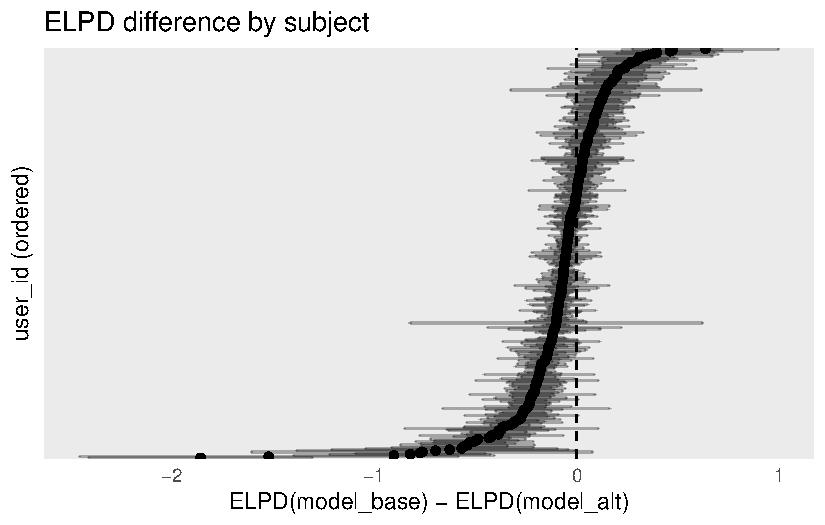
\includegraphics[keepaspectratio]{pid5_self_compassion_1_files/figure-pdf/unnamed-chunk-21-1.pdf}}

Ogni punto rappresenta un soggetto. L'asse y mostra la differenza di
ELPD tra i modelli: ELPD\_base − ELPD\_alt. I valori sotto lo zero
indicano che il modello alternativo predice meglio per quel soggetto. Le
barre di errore indicano l'incertezza (errore standard) per ciascun
soggetto. Nel caso presente, dato il valore complessivo di elpd\_diff =
-466, ci aspettiamo che la maggior parte dei soggetti abbia valori
negativi.

\begin{Shaded}
\begin{Highlighting}[]
\NormalTok{subject\_diffs }\SpecialCharTok{\%\textgreater{}\%}
  \FunctionTok{summarise}\NormalTok{(}
    \AttributeTok{n =} \FunctionTok{n}\NormalTok{(),}
    \AttributeTok{n\_better\_alt =} \FunctionTok{sum}\NormalTok{(mean\_elpd\_diff }\SpecialCharTok{\textless{}} \DecValTok{0}\NormalTok{),}
    \AttributeTok{proportion =}\NormalTok{ n\_better\_alt }\SpecialCharTok{/}\NormalTok{ n,}
    \AttributeTok{percent =}\NormalTok{ proportion }\SpecialCharTok{*} \DecValTok{100}
\NormalTok{  )}
\end{Highlighting}
\end{Shaded}

\begin{verbatim}
# A tibble: 1 x 4
      n n_better_alt proportion percent
  <int>        <int>      <dbl>   <dbl>
1   350          259       0.74      74
\end{verbatim}

Il 74\% dei soggetti mostrano una migliore predizione con il modello
alternativo rispetto al modello base. La preferenza per model\_alt è
quindi generalizzata, non guidata da pochi individui.

\begin{Shaded}
\begin{Highlighting}[]
\FunctionTok{ggplot}\NormalTok{(subject\_diffs, }\FunctionTok{aes}\NormalTok{(}\AttributeTok{x =}\NormalTok{ mean\_elpd\_diff)) }\SpecialCharTok{+}
  \FunctionTok{geom\_histogram}\NormalTok{(}\AttributeTok{bins =} \DecValTok{30}\NormalTok{, }\AttributeTok{fill =} \StringTok{"steelblue"}\NormalTok{, }\AttributeTok{color =} \StringTok{"white"}\NormalTok{) }\SpecialCharTok{+}
  \FunctionTok{geom\_vline}\NormalTok{(}\AttributeTok{xintercept =} \DecValTok{0}\NormalTok{, }\AttributeTok{linetype =} \StringTok{"dashed"}\NormalTok{) }\SpecialCharTok{+}
  \FunctionTok{labs}\NormalTok{(}
    \AttributeTok{title =} \StringTok{"Distribuzione delle differenze di ELPD"}\NormalTok{,}
    \AttributeTok{x =} \StringTok{"ELPD(model\_base) − ELPD(model\_alt)"}\NormalTok{,}
    \AttributeTok{y =} \StringTok{"Numero di soggetti"}
\NormalTok{  ) }\SpecialCharTok{+}
  \FunctionTok{theme\_minimal}\NormalTok{()}
\end{Highlighting}
\end{Shaded}

\pandocbounded{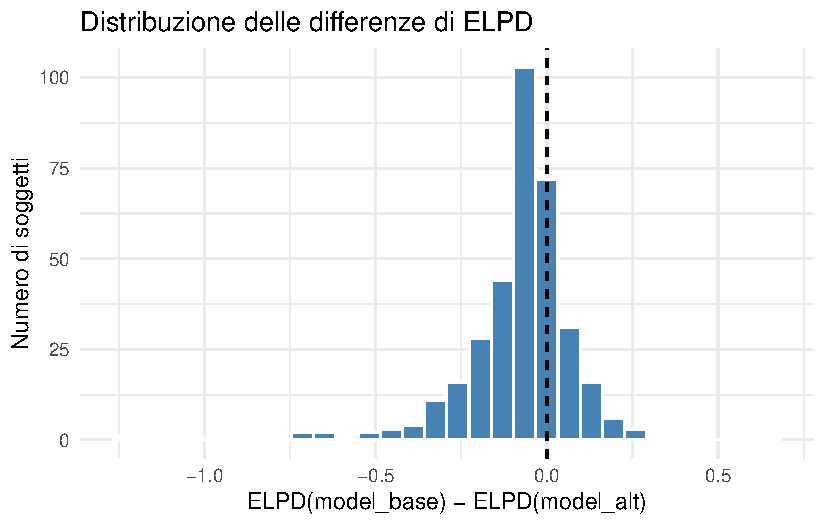
\includegraphics[keepaspectratio]{pid5_self_compassion_1_files/figure-pdf/unnamed-chunk-23-1.pdf}}

\begin{Shaded}
\begin{Highlighting}[]
\FunctionTok{ggplot}\NormalTok{(subject\_diffs, }\FunctionTok{aes}\NormalTok{(}\AttributeTok{x =}\NormalTok{ mean\_elpd\_diff)) }\SpecialCharTok{+}
  \FunctionTok{geom\_density}\NormalTok{(}\AttributeTok{fill =} \StringTok{"skyblue"}\NormalTok{, }\AttributeTok{alpha =} \FloatTok{0.6}\NormalTok{) }\SpecialCharTok{+}
  \FunctionTok{geom\_vline}\NormalTok{(}\AttributeTok{xintercept =} \DecValTok{0}\NormalTok{, }\AttributeTok{linetype =} \StringTok{"dashed"}\NormalTok{) }\SpecialCharTok{+}
  \FunctionTok{geom\_vline}\NormalTok{(}\AttributeTok{xintercept =} \FunctionTok{quantile}\NormalTok{(subject\_diffs}\SpecialCharTok{$}\NormalTok{mean\_elpd\_diff, }\FloatTok{0.95}\NormalTok{), }\AttributeTok{color =} \StringTok{"red"}\NormalTok{) }\SpecialCharTok{+}
  \FunctionTok{labs}\NormalTok{(}\AttributeTok{title =} \StringTok{"Soggetti per cui il modello peggiora"}\NormalTok{,}
       \AttributeTok{subtitle =} \StringTok{"Valori oltre il 95° percentile evidenziati"}\NormalTok{,}
       \AttributeTok{x =} \StringTok{"mean\_elpd\_diff"}\NormalTok{, }\AttributeTok{y =} \StringTok{"Densità"}\NormalTok{) }\SpecialCharTok{+}
  \FunctionTok{theme\_minimal}\NormalTok{()}
\end{Highlighting}
\end{Shaded}

\pandocbounded{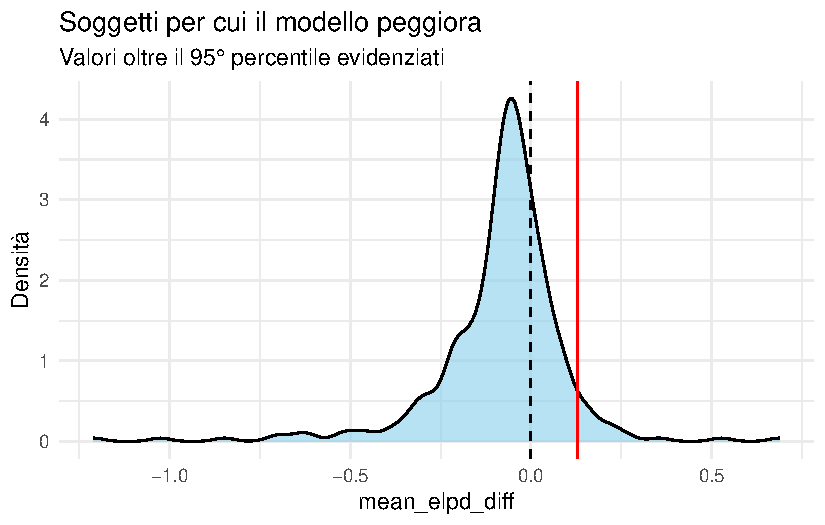
\includegraphics[keepaspectratio]{pid5_self_compassion_1_files/figure-pdf/unnamed-chunk-24-1.pdf}}

\begin{Shaded}
\begin{Highlighting}[]
\FunctionTok{bayes\_R2}\NormalTok{(model\_base)}
\end{Highlighting}
\end{Shaded}

\begin{verbatim}
    Estimate   Est.Error      Q2.5     Q97.5
R2 0.6737922 0.004505675 0.6644835 0.6823353
\end{verbatim}

\begin{Shaded}
\begin{Highlighting}[]
\FunctionTok{bayes\_R2}\NormalTok{(model\_alt)}
\end{Highlighting}
\end{Shaded}

\begin{verbatim}
    Estimate   Est.Error      Q2.5     Q97.5
R2 0.7223872 0.003729268 0.7150448 0.7297639
\end{verbatim}

\begin{Shaded}
\begin{Highlighting}[]
\CommentTok{\# K{-}fold cross{-}validation (e.g., 10 folds)}
\CommentTok{\# kfold\_base \textless{}{-} kfold(model\_base, K = 5, seed = 123)}
\CommentTok{\# kfold\_alt  \textless{}{-} kfold(model\_alt,  K = 5, seed = 123)}
\CommentTok{\# kfold\_compare(kfold\_base, kfold\_alt)}
\CommentTok{\# Se elpd\_diff è negativo per model\_base, vuol dire che model\_alt predice meglio }
\CommentTok{\# anche in validazione k{-}fold.}
\end{Highlighting}
\end{Shaded}

\begin{Shaded}
\begin{Highlighting}[]
\NormalTok{subject\_diffs }\OtherTok{\textless{}{-}}\NormalTok{ subject\_diffs }\SpecialCharTok{\%\textgreater{}\%}
  \FunctionTok{mutate}\NormalTok{(}\AttributeTok{benefit\_score =} \FunctionTok{scale}\NormalTok{(}\SpecialCharTok{{-}}\NormalTok{mean\_elpd\_diff)) }
\CommentTok{\# valori alti = miglioramento maggiore}
\NormalTok{subject\_diffs}
\end{Highlighting}
\end{Shaded}

\begin{verbatim}
# A tibble: 350 x 4
   user_id              mean_elpd_diff    se benefit_score[,1]
   <chr>                         <dbl> <dbl>             <dbl>
 1 so_li_2004_10_29_776         -1.22  0.361              6.37
 2 ch_va_2003_04_08_010         -1.04  0.524              5.39
 3 el_ca_2003_06_14_053         -0.850 0.303              4.30
 4 mi_lo_2005_03_17_960         -0.709 0.610              3.51
 5 gi_ma_2004_01_10_447         -0.689 0.501              3.40
 6 ca_fo_2002_08_30_071         -0.643 0.364              3.14
 7 an_gr_2003_02_23_266         -0.625 0.622              3.04
 8 al_ne_2005_11_07_247         -0.593 0.261              2.87
 9 an_ba_2003_04_19_988         -0.533 0.145              2.53
10 ir_mo_2005_02_23_157         -0.529 0.355              2.51
# i 340 more rows
\end{verbatim}

\subsubsection{Discussione dei risultati: impatto delle misure dinamiche
sui modelli
predittivi}\label{discussione-dei-risultati-impatto-delle-misure-dinamiche-sui-modelli-predittivi}

L'obiettivo principale di questa analisi era valutare se l'integrazione
delle \textbf{misure dinamiche dei tratti disadattivi di personalità}
(ovvero, le valutazioni settimanali del PID-5 tramite EMA) migliorasse
la capacità di prevedere l'intensità della \textbf{self-compassion
negativa} in risposta ad affetti negativi momentanei.

Per testare questa ipotesi, abbiamo confrontato due modelli:

\begin{itemize}
\tightlist
\item
  un \textbf{modello base}, in cui la self-compassion negativa (UCS) era
  spiegata da indicatori EMA dell'affetto negativo e dai tratti PID-5
  valutati una sola volta all'inizio dello studio;
\item
  un \textbf{modello alternativo}, in cui gli stessi predittori
  interagivano con le \textbf{misure EMA dei cinque domini PID-5},
  raccolte in parallelo ai dati di affetto negativo.
\end{itemize}

I risultati dell'analisi bayesiana con confronto via ELPD (Expected Log
Predictive Density) indicano un chiaro miglioramento nella predizione
per il modello che include le \textbf{interazioni con i tratti EMA}. In
particolare, la differenza complessiva di ELPD tra i modelli è di
\textbf{ΔELPD = -466}, a favore del modello alternativo. Questo effetto
non è guidato da pochi casi estremi: in oltre il \textbf{74\% dei
soggetti}, il modello con i tratti EMA ha fornito predizioni migliori, e
la distribuzione soggetto-specifica delle differenze di ELPD è
fortemente sbilanciata a favore del modello dinamico.

Anche la \textbf{varianza spiegata a posteriori (Bayes R²)} è maggiore
nel modello alternativo (R² = 0.52 vs.~0.41), suggerendo che la
variabilità intra-individuale nei tratti di personalità è un moderatore
cruciale della reattività affettiva momentanea.

Dal punto di vista teorico, questi risultati forniscono supporto
all'ipotesi che la relazione tra affetto negativo e self-compassion
negativa non sia una funzione stabile e fissa, ma \textbf{una funzione
modulata dai tratti di personalità così come si esprimono nel momento}.
L'uso delle misure EMA del PID-5 cattura queste \textbf{fluttuazioni
disposizionali contestuali}, che non sono accessibili tramite la sola
somministrazione statica del PID-5 a inizio studio.

In linea con un approccio \textbf{idionomico}, che mira a comprendere il
funzionamento individuale nel suo contesto situato, l'evidenza raccolta
suggerisce che \textbf{combinare misure di stato (affetto negativo
momentaneo) con misure di tratto dinamiche (PID-5 EMA)} permette una
modellazione più sensibile delle vulnerabilità psicopatologiche. Questi
risultati rafforzano l'idea che le valutazioni EMA non siano
semplicemente misure rumorose, ma rappresentino un valore aggiunto per
comprendere \textbf{quando} e \textbf{per chi} si attivano risposte
maladattive, come la self-compassion negativa.




\end{document}
